\documentclass[notes]{subfiles}

\begin{document}
	\addcontentsline{toc}{section}{4.2 - The Definite Integral}
	\refstepcounter{section}
	\fancyhead[RO,LE]{\bfseries \large\nameref{cs42}} 
	\fancyhead[LO,RE]{\bfseries \currentname}
	\fancyfoot[C]{{}}
	\fancyfoot[RO,LE]{\large \thepage}	%Footer on Right \thepage is pagenumber
	\fancyfoot[LO,RE]{\large Chapter 4.2}
	
\section*{The Definite Integral} \label{cs42}
	\subsection*{Before Class}
	\addcontentsline{toc}{subsection}{Before Class}
	\subsubsection*{Definition}
	\addcontentsline{toc}{subsubsection}{Definition}
		\begin{defn}[Definite Integral]
			Let $f$ be a function defined for $a\leq x\leq b$, and divide $[a,b]$ into $n$ subintervals of width $\Delta x = \dfrac{b-a}{n}$.  Let 
				\[a=x_0,x_1,x_2,...,x_{n-1},x_n=b\]
			be the endpoints of these subintervals, and let $x_i^*$ be any sample points in these subintervals, so that $x_i^*$ lies in the $i$th subinterval $[x_{i-1},x_i]$.  Then, the \textbf{definite integral of f from a to b} is given by
				\showto{ins}{
					\[\int_a^b f(x)\, dx = \lim_{n\to\infty} \sum_{i=1}^n f(x_i^*)\Delta x\]
				}
				\showto{st}{
					\vspace{.75in}\\
				}
			provided that this limit exists and gives the same value for all possible choices of sample points.  If it does exist, we say that $f$ is \textbf{integrable} on $[a,b]$.\\ \\ \\
			
			The sum 
				\showto{ins}{
					$\ds \sum_{i=1}^n f(x_i^*)\Delta x$
				}
				\showto{st}{
					\blank{2.5}
				} 
			is called a \textbf{Riemann sum}.  		
		\end{defn}
		
		\begin{rmk}[Terminology]
			\showto{ins}{
				Given the definite integral $\ds \int_a^b f(x)\, dx$, we have some terminology:
				\begin{itemize}
					\item $a$ is called the \emph{lower bound/limit (of integration)}
					\item $b$ is called the \emph{upper bound/limit (of integration)}
					\item $\ds \int$ is called an \emph{integral sign}
					\item We use $dx$ to denote an infinitesimal change in $x$.
				\end{itemize}
			}
			\showto{st}{ 
				Given the definite integral $\ds \int_a^b f(x)\, dx$, we have some terminology:\\ \\
				\begin{itemize}
				\setlength\itemsep{30pt}
					\item $a$ is called the \blank{5}
					\item $b$ is called the \blank{5}
					\item $\ds \int$ is called an \blank{3}
					\item We use $dx$ to denote an \blank{4}
				\end{itemize}
			}
		\end{rmk}
			\newpage
			
		\begin{rmk}[Theorem]
			\showto{ins}{
				If $f$ is continuous on $[a,b]$, or if $f$ has only a finite number of jump discontinuities, then $f$ is integrable on $[a,b]$.
			}
			\showto{st}{
				If $f$ is continuous on $[a,b]$, or if $f$ has \blank{3.8},\vspace{20pt} then \blank{4}.			
			}
		\end{rmk}
		
		\begin{rmk}[Theorem]
			\showto{ins}{
				If $f$ is integrable on $[a,b]$, then
					\[\int_a^b f(x)\, dx = \lim_{n\to\infty} \sum_{i=1}^n f(x_i)\Delta x\]
				where $\Delta x= \dfrac{b-a}{n}$ and $x_i = a + i\Delta x$.
			}
			\showto{st}{
				If $f$ is integrable on $[a,b]$, then\vspace{1in} \\
				
			}
		\end{rmk}
		
		\begin{rmk}[Interpretation of the Integral]
			The definite integral $\ds \int_a^b f(x)\, dx$ can be interpreted as\vspace{5pt}
			\showto{ins}{
				\begin{itemize}
					\item The \emph{total} area between the $f(x)$ and the $x-$axis if $f(x) \geq 0$ on $[a,b]$
					\item The \emph{net} area between $f(x)$ and the $x-$axis if $f(x)$ takes on positive and negative values on $[a,b]$			
				\end{itemize}
			}
			\showto{st}{
				\begin{itemize}
				\setlength\itemsep{30pt}
					\item The \emph{total} area between the $f(x)$ and the $x-$axis if \blank{2.5}
					\item The \emph{net} area between $f(x)$ and the $x-$axis if \blank{2.7}\vspace{20pt} \blank{4}
				\end{itemize}
			}
		\end{rmk}
		Here are some pictures to help with the interpretations:
			\vs{1}

			\newpage
			
		\begin{ex}
			Express $\ds \lim_{n\to \infty} \sum_{i = 1}^n \lrpar{x_i^3 - 2x_i^2 + 1 - x_i\cos(x_i)}\Delta x$ as an integral.  Use proper notation.
		\end{ex}
			\vs{1}
			
		\begin{ex}
			\begin{enumerate}[(a)]
				\item The greatest integer function $\llbracket x \rrbracket$ is integrable on any finite-length interval, but not necessarily differentiable on the same interval.  Why is this consistent with the above information?
					\vs{1}
					
				\item Compute $\ds \int_0^5 \llbracket x \rrbracket\, dx$, \emph{using geometry}.
					\vs{1}
			
			\end{enumerate}
		\end{ex}
			\newpage
	
	\subsubsection*{Pre-Class Activities}	
	\addcontentsline{toc}{subsubsection}{Pre-Class Activities}		
		\begin{ex}
			The shaded area on the graphs of $\sin x$ and $\cos x$ are both exactly 1.  
			\begin{center}
				\begin{tikzpicture}
					\begin{axis}[
						width = .5\textwidth,
						every tick label/.append style={font=\scriptsize},
						axis x line = middle,
						axis y line = middle,
						grid = both,
						grid style={line width=.1pt, draw=gray!10},
						major grid style={line width=.2pt,draw=gray!50},
						minor grid style={line width=.2pt, draw=gray!40},
			    			every axis y label/.style={at={(ticklabel cs:1.15)}},
			    			%ytick = {-4, -2, -3, -1, 1, 2, 3, 4},
			    			ymin = -1, ymax = 1,
						y label style={at={(axis description cs:.5,1.15)},anchor=north},
			    			ylabel = {$\sin x$},
		    				every axis x label/.style= {at ={(ticklabel cs:1)}},
		    				xtick = {-7.85, -6.28, -4.71, -3.14,- 1.57,  0, 1.57, 3.14, 4.71, 6.28, 7.85},
		    				x label style={at={(axis description cs:1.1,.5)},anchor=east},
		    				xticklabels = {$-\dfrac{5\pi}{2}$, $-2\pi$, $-\dfrac{3\pi}{2}$, $-\pi$, $-\dfrac{\pi}{2}$,0,$\dfrac{\pi}{2}$, $\pi$, $\dfrac{3\pi}{2}$, $2\pi$, $\dfrac{5\pi}{2}$},
		    				xlabel = {$x$},
		    				xmin = -10, xmax = 10
		    				%minor y tick num = 2,
					]
					
					\addplot[thick,smooth, samples = 100, domain = -10:10, name path = A] {sin(deg(x))};
					\addplot[draw = none, name path = B, domain = 0:1.57] {0};
					\addplot[gray] fill between[of = A and B, soft clip = {domain = 0:1.57}];
					\end{axis}
				\end{tikzpicture}
				\begin{tikzpicture}
					\begin{axis}[
						width = .5\textwidth,
						every tick label/.append style={font=\scriptsize},
						axis x line = middle,
						axis y line = middle,
						grid = both,
						grid style={line width=.1pt, draw=gray!10},
						major grid style={line width=.2pt,draw=gray!50},
						minor grid style={line width=.2pt, draw=gray!40},
			    			every axis y label/.style={at={(ticklabel cs:1.15)}},
			    			%ytick = {-4, -2, -3, -1, 1, 2, 3, 4},
			    			ymin = -1, ymax = 1,
						y label style={at={(axis description cs:.5,1.15)},anchor=north},
			    			ylabel = {$\cos x$},
		    				every axis x label/.style= {at ={(ticklabel cs:1)}},
		    				xtick = {-7.85, -6.28, -4.71, -3.14,- 1.57,  0, 1.57, 3.14, 4.71, 6.28, 7.85},
		    				x label style={at={(axis description cs:1.1,.5)},anchor=east},
		    				xticklabels = {$-\dfrac{5\pi}{2}$, $-2\pi$, $-\dfrac{3\pi}{2}$, $-\pi$, $-\dfrac{\pi}{2}$,0,$\dfrac{\pi}{2}$, $\pi$, $\dfrac{3\pi}{2}$, $2\pi$, $\dfrac{5\pi}{2}$},
		    				xlabel = {$x$},
		    				xmin = -10, xmax = 10
		    				%minor y tick num = 2,
					]
					
					\addplot[thick,smooth, samples = 100, domain = -10:10, name path = A] {cos(deg(x))};
					\addplot[draw = none, name path = B, domain = 0:1.57] {0};
					\addplot[gray] fill between[of = A and B, soft clip = {domain = 0:1.57}];
					\end{axis}
				\end{tikzpicture}
			\end{center}
			\begin{enumerate}[(a)]
				\item Compute the \emph{net area} of $\sin x$ on the interval $[0,2\pi]$.
					\vs{1}
					
				\item Compute the \emph{total area} of $\sin x$ on the interval $[0,2\pi]$.
					\vs{1}
					
				\item Compute the \emph{net area} of $\cos x$ on the interval $\left[-\dfrac{3\pi}{2}, \pi\right]$.
					\vs{1}
					
				\item Compute the \emph{total area} of $\cos x$ on the interval $\left[-\dfrac{3\pi}{2}, \pi\right]$.
					\vs{1}
					
				\item Compute the \emph{net area} of $\sin x$ on the intervals $\left[-\dfrac{\pi}{2},\dfrac{\pi}{2}\right]$ and $[-\pi,\pi]$.  What conjecture can you make about the net area of odd functions over symmetric intervals?
					\vs{1}
					
				\item Compute the \emph{net area} of $\cos x$ on the intervals $\left[-\dfrac{\pi}{2},\dfrac{\pi}{2}\right]$ and $[-\pi,\pi]$.  What conjecture can you make about the net area of even functions over symmetric intervals?
					\vs{1}
			\end{enumerate}
		\end{ex}
			\newpage
			
	\subsection*{In-Class}
	\addcontentsline{toc}{subsection}{In-Class}
	\subsubsection*{Evaluating Integrals}
	\addcontentsline{toc}{subsubsection}{Evaluating Integrals}
		\begin{ex}
			Use the definition of the definite integral to show that $\ds \int_2^4 x\, dx = 6$.
		\end{ex}
			\vs{3}
			
		\showto{ins}{
			\begin{center}
				\tabulinesep = 4mm
				{\setlength{\arrayrulewidth}{1.5pt}
				\begin{tabu}{| X[l] X[l] | X[l] X[l] |}\hline
					\multicolumn{2}{|c|}{\large{\textbf{Helpful Formulas}}} & \multicolumn{2}{c|}{\large{\textbf{Rules for Sigma Notation}}} \\
					 $\ds \sum_{i=1}^n i$ & $ \dfrac{n(n+1)}{2}$	& $\ds \sum_{i=1}^n c = $	& $nc$ \\ 
					 $\ds \sum_{i=1}^n i^2$ & $\dfrac{n(n+1)(2n+1)}{6}$	& $\ds \sum_{i=1}^n ca_i$	& $c\ds\sum_{i=1}^n a_i$ \\
					 $\ds \sum_{i=1}^n i^3$ & $\lrpar{\dfrac{n(n+1)}{2}}^2$	& $\ds \sum_{i=1}^n (a_i\pm b_i)$ & $\ds\sum_{i=1}^n a_i \pm \sum_{i=1}^n b_i$ \\ \hline
				\end{tabu}
				}
			\end{center}
		}
		\showto{st}{			
			\begin{center}
				\tabulinesep = 4mm
				{\setlength{\arrayrulewidth}{1.5pt}
				\begin{tabu}{| X[l] X[c] | X[l] X[c] |}\hline
					\multicolumn{2}{|c|}{\large{\textbf{Helpful Formulas}}} & \multicolumn{2}{c|}{\large{\textbf{Rules for Sigma Notation}}} \\
					 $\ds \sum_{i=1}^n i$ & 	& $\ds \sum_{i=1}^n c  $	&  \\ 
					 $\ds \sum_{i=1}^n i^2$ & 	& $\ds \sum_{i=1}^n ca_i$	&  \\
					 $\ds \sum_{i=1}^n i^3$ & 	& $\ds \sum_{i=1}^n (a_i\pm b_i)$ &  \\ \hline
				\end{tabu}
				}
			\end{center}
		}
			\newpage
			
		\begin{ex}
			Evaluate $\ds \int_0^3 (x^3-2x)\,dx$ using the definition of the definite integral.
		\end{ex}
			\newpage
			
		\begin{ex}
			Set up an expression for $\ds\int_2^5 x^4\, dx$ as a limit of sums.
		\end{ex}
			\vs{1}
			
		\begin{ex}
			The graph of $f$ is given below.\\
			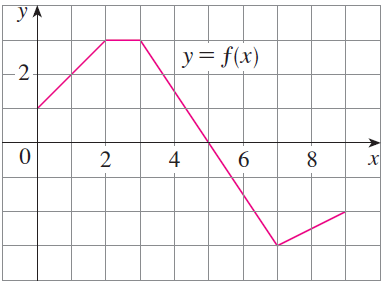
\includegraphics{4.2fig1}\\
			Evaluate each integral by interpreting it in terms of areas.
			\begin{enumerate}[(a)]
				\item $\ds \int_0^2 f(x)\, dx$
					\vs{1}
					
				\item $\ds \int_0^5 f(x)\, dx$
					\vs{1}
					
				\item $\ds \int_5^7 f(x)\, dx$
					\vs{1}
					
				\item $\ds \int_0^9 f(x)\, dx$
					\vs{1}
			\end{enumerate}
		\end{ex}
			\newpage
			
	\subsubsection*{The Midpoint Rule}
	\addcontentsline{toc}{subsubsection}{The Midpoint Rule}
		Instead of choosing our sample points to be left or right endpoints, we can choose any point inside the subinterval; a standout is the midpoint of the interval.  
			\begin{defn}[Midpoint Rule]
				\showto{ins}{
					\[\int_a^b f(x)\,dx\approx \sum_{i=1}^n f(\overline{x_i})\Delta x\]
					where $\Delta x = \dfrac{b-a}{n}$ and $\overline{x_i} = \dfrac{x_{i-1}+x_i}{2}$ is the midpoint of the interval $[x_{i-1},x_i]$.
				}
				\showto{st}{
					$ $\vspace{1in}\\ \\ 
				}
			\end{defn}
			
		\begin{ex}
			Use the Midpoint Rule with $n = 5$ to approximate $\ds \int_1^2 \dfrac{1}{x}\, dx$
		\end{ex}
			\vs{1.5}
			\newpage
			
	\subsubsection*{Properties of the Definite Integral}	
	\addcontentsline{toc}{subsubsection}{Properties of the Definite Integral}
		The following are useful properties when working with the definite integral:
			\begin{thm}[Properties of the Definite Integral]
				 Let $f,g$ be continuous functions on $[a,b]$.  Let $c$ be a constant.  Then,
				\showto{ins}{
					\begin{enumerate}[(1)]
						\item $\ds \int_a^b f(x)\,dx = -\int_b^a f(x)\, dx$
						\item $\ds \int_a^a f(x)\,dx = 0$
						\item $\ds \int_a^b c\, dx = c(b-a)$
						\item $\ds \int_a^b [f(x)\pm g(x)]\,dx = \int_a^b f(x)\,dx\pm \int_a^b g(x)\,dx$
						\item $\ds \int_a^b cf(x)\,dx = c\int_a^b f(x)\,dx$
						\item $\ds \int_a^b f(x)\, dx = \int_a^d f(x)\, dx + \int_d^b f(x)\, dx$, for some $a < d < b$.
					\end{enumerate}
				}
				\showto{st}{ \\
					\begin{enumerate}[(1)]
					\setlength\itemsep{35pt}
						\item 
						\item 
						\item 
						\item 
						\item 
						\item 
					\end{enumerate}
				}
			\end{thm}
		
		\begin{ex}
			If $\ds \int_0^6 f(x)\, dx = 10$ and $\ds \int_0^8 f(x)\, dx = 4$, what is $\ds\int_6^8 f(x)\, dx$?
		\end{ex}	
			\vs{1.5}
			\newpage
	
		\begin{ex}
			Compute $\ds \int_1^2 (4+2x^2)\,dx$.
		\end{ex}
			\vs{1}

		\begin{ex}
			For any $a,b$, find the value of $\ds \int_a^b x\, dx$ 			
		\end{ex}
			\vs{1}
			\newpage
			
		\begin{ex}
			Evaluate the integrals by interpreting them in terms of area:
			\begin{enumerate}[(a)]
				\item $\ds \int_0^9 \lrpar{\dfrac{2}{3}x - 2}\, dx$
					\vs{1}
					
				\item $\ds \int_{-6}^6 \lrpar{x - \sqrt{36-x^2}}\, dx$
					\vs{1}
					
				\item $\ds \int_0^1 |2x - 1|\, dx$
					\vs{1}
			\end{enumerate}
		\end{ex}
			\newpage 
	\subsection*{After Class}	
	\addcontentsline{toc}{subsection}{After Class}
		
		\begin{ex}
			If $\ds \int_0^9 f(x)\, dx = 37$ and $\ds \int_0^9 g(x)\, dx = 16$, what is $\ds \int_0^9 \lrpar{2f(x) + 3g(x)}\, dx$?
		\end{ex}
			\vs{1}
			
		\begin{ex}
			Use the definition of the integral to find $\ds \int_1^4 \lrpar{x^2 - 4x + 2}\, dx $
		\end{ex}
			\vs{2}
			\newpage 

		\begin{ex}
			Use the Midpoint Rule to estimate $\ds \int_0^1 \sqrt{x^3+1}\, dx$ to four decimal places, using $n = 5$ rectangles.
		\end{ex}
			\vs{1}
			
		\begin{ex}
			If $\ds \int_0^\pi \sin^4 x\, dx = \dfrac{3\pi}{8}$, what is $\ds \int_\pi^0 \sin^4 x\, dx$?  Why?
		\end{ex}
			\vs{1}
	\clearpage
\end{document}